\documentclass[12pt]{article}

\usepackage{graphicx}
\graphicspath{ {./images/} }

\usepackage[slovak]{babel}

\begin{document}\begin{titlepage}
    \vspace*{\fill}
    \begin{center}
      {\LARGE Klasifikácia Phishigových Mailov}\\[0.25cm]
      {\Large Daniel Trizna}\\
    \end{center}
    \vspace*{\fill}
  \end{titlepage}
\newpage

\section*{Abstrakt}
V tomto dokumente sa budeme venovať riešeniu problematiky rozoznávania phishingových emailov od bežnej mailovej komunikácie. Na toto rozoznávanie budeme používať strojové učenie.\\

Phishing je spôsob útoku prostrednítvom elektronickej komunikácie, pomocou ktorého sa útočník snaží svoju obeť podviesť tak, aby od nej získal osobné informácie, prípadne platobné údaje, ktoré sa následne útočník pokúsi zneužiť.\\

V nasledujúcich častiach sa budeme venovať dátam s ktorými pracujeme a ich spracovaniu. Ďalej sa budeme venovať metódam, ktoré sme na klasifikáciu phishingových mailov použili a ich výsledkom na našich dátach.

\section*{Opis problému}
V tomto projekte riešime problematiku klasifikácie dát. Naše dáta predstavujú jednotlivé maily, ktoré môžu spadať do kategórie bežnej elektronickej komunikácie a maily, ktoré spadajú do kategórie phishingových mailov. Táto klasifikácie môže byť následne využitá na filtrovanie elektronickej pošty, prípadne na upozornenie používateľa na možné riziko phishingového útoku a na to aby zvýšil svoju ostražitosť. Strojové učenie v tejto problematike bolo využité už v niekoľkých publikáciach ako napríklad Classification of Phishing Email Using Random Forest Machine Learning Technique(Andronicus A. Akinyelu, Aderemi O. Adewumi) alebo Detection of Phishing Attacks: A Machine Learning Approach (Ram Basnet, Srinivas Mukkamala, and Andrew H. Sung). Tieto články poskytujú zaujímavý pohľad na túto problematiku rovnako ako na jej riešenie.

\section*{Dáta}
Ako zdroj našich dát sme využili dva verejne dostupné korpusy, jeden pozostávajúci z čisto phishingových mailov a druhý pozostávaúci z bežnej komunikácie.
\subsubsection*{Korpus phishingových mailov}
Tento korpus pozostáva zo 4548 phishingových mailov, ktoré sú vo formáte .eml. Tieto maily obsahujú odosielateľa, príjemcu, telo mailu rovnako ako aj prílohy. Tieto maily budú využité ako pozitívne príklady pri učení rovnako ako aj pri testovaní. Tento korpus je dostupný na academictorrents.com pod názvom Phishing corpus.
\subsubsection*{Korpus bežnej mailovej komunikácie}
Tento korpus pozostáva z mailovej komunikácie vyše 150 používateľov a obsahuje okolo pol milióna správ. Tieto maily majú rovnakú štruktúru ako maily v korpuse phishingových mailov. Tento dataset je verejne dostupný na stránke academictorrents.com pod názvom Enron Email Dataset.\\

Keďže máme k dispozícii omnoho väčšie kvantum bežnej mailovej komunikácie v pomere k phishingovým mailom, budeme musieť využiť iba časť korpusu bežnej mailovej komunikácie. V prípade, že by sme využili celý korpus bežnej mailovej komunikácie náš model by mal problém sa čokolvek naučiť nakoľko keby zakaždým povedal, že to nie je phishingový mail dosahoval by úspešnosť viac ako 90\%. Ako dataset budeme využívať príklady v pomere 1:2 (pozitívne k negatívnym).

\section*{Preprocessing}
Na to aby sme mohli na náš problém využiť strojové učenie je potrebné naše trénovacie dáta najprv spracovať a vybrať z nich charakteristické vlastnosti na základe ktorých by bol počítač schopný rozoznávať škodlivé maily od neškodných. Charakteristické vlastnosti (features) sme v našom projekte zvolili nasledovné:
\begin{itemize}
\item \textbf{URL obsahujúce IP adresu} - vieme, že bežné webstránky v svojej adrese neobsahujú čistú IP adresu ale názov danej domény - ak mail obsahuje link tvaru http://142.251.36.142 namiesto https://www.google.com/ tak mu priradíme vlastnosť s hodnotou 1 inakšie mu priradíme hodnotu 0

\item \textbf{Rozdielna adresa v odkaze a v texte} - Maily je možné posielať aj vo formáte html, kde sa môžu nachádzať rôzne html tagy. Jedným z týchto tagov je \textit{a}, ktorý slúži na odkazovanie na externé stránky. Tag \textit{a} má vlastnosť \textit{href}, ktorá hovorí o tom, na ktorú stránku nás daný tag presmeruje. Vo vnútri samotného tagu je potom text, na ktorý keď klikneme budeme presmerovaný na danú stránku. V prípade že sa v maily nachádza tag typu : $<$a href="facebook.com"$>$google.com$<$/a$>$, kde adresa vo vnútri tagu nezodpovedá tej, na ktorú nás link presmeruje priradíme tomuto mailu vlastnosť s hodnotou 1 inak mu priradíme vlastnosť s hodnotou 0.

\item \textbf{Veľký počet bodiek v adrese} - Vieme, že ak nejaká adresa v maily obsahuje viac ako 3 bodky je väčšia pravdepodobnosť že táto adresa smeruje na potenciálne škodlivú stránku a teda mail má veľkú pravdepodobnosť, že spadá do kategórie phishingových mailov.

\item \textbf{Nezhoda domény odosielateľa s doménou v odkazoch} - Pokiaľ sa v maily nachádza viacero rôznych odkazov, kde každý z nich odkazuje na stránku s inou doménou ako je tá, z ktorej je odoslaný daný mail, tento mail má vyššiu pravdepodobnosť byť pokusom o phishing. Napríklad ak bol mail odoslaný z adresy podpora@nbs.sk ale v samotnom tele mailu sa nachádzajú linky typu scam.com/nbs vieme, že tento mail je potenciálna hrozba. Teda mailu priradíme ďalšiu vlastnosť hovoriacu o tom koľko adries s rôznou doménou sa v danom maily nachádza.

\item \textbf{Typ textu mailu} - Ako sme už vyššie spomenuli, niektoré maily môžu obsahovať aj html notáciu. Maily s html notáciou majú vo všeobecnosti vyššiu pravdepodobnosť na to aby boli potenciálne škodlivé a teda každému mailu priradíme 1 v prípade že jeho text obsahuje html notáciu a 0 v prípade, že nie.

\item \textbf{Javascript v maily} - Keďže vieme, že mail môže obsahovať html notáciu, môže taktiež obsahovať aj malé kúsky javascriptového kódu, ktorý môže byť potenciálne nebezpečný. Teda v prípade, že mail obsahuje tag script alebo inú formu javascriptu tomuto mailu priradíme vlastnosť s hodnotou 1 inakšie bude mať hodnotu 0.

\item \textbf{Obsah slov z určitej kategórie} - Vieme, že phishingové útoky využívajú väčšinou podobné stratégie. Buď sa snažia používateľa presvedčiť o verifikáciu jeho účtu, o prihlásenie do jeho účtu alebo o potvrdenie nejakej transakcie alebo čohokoľvek iného. Preto sme pridali tri ďalšie vlastnosti, ktoré hovoria o tom či daný mail spadá do dákej z týchto kategórii podľa toho či obsahuje niektoré z týchto slov:
\begin{itemize}
\item \textbf{verifikácia účtu} - \textit{verify}, \textit{account}, \textit{notify}, \textit{credentials} 
\item \textbf{prihlásenie do účtu} - \textit{login}, \textit{username}, \textit{password},  \textit{click}
\item \textbf{potvrdenie} - \textit{update}, \textit{confirm}
\end{itemize}
\end{itemize}

\section*{Prístupy a ich výsledky}
V nasledujúcej časti sa budem venovať prístupom, ktoré som na riešenie tohto klasifikačného problému zvolil rovnako ako aj ich výsledkom. Na ohodnotenie jednotlivých prístupov sme využívali testovaciu množinu, ktorú sme vyčlenili z nášho pôvodného datasetu. Na porovnanie výsledkov sme využili základnú baseline, ktorá nám vrátila najčastejšiu hodnotu.

\subsubsection*{Support Vector Classification}
Ako prvý prístup sme vyskúšali Support Vector Classification (SVC). S týmto prístupom sme sa streti v priebehu cvičení, kde sme sa dozvedeli, že má niekoľko parametrov, ktoré vieme doladiť aby sme ho napasovali čo najlepšie na náš problém. Experimentálne sme prišli na to, že najlepšie výsledky tento prístup dosahoval s rbf kernelom a s hodnotami C rovnými 2 a gamma rovnou 1. Pre baseline s úspešnosťou 65\% dosahoval tento klasifikátor 95\% úspešnosť a teda našu chybu sme zredukovali o necelých 86\%.

\subsubsection*{Random Forest Classifier}
Ďalší prístup, ktorý sme vyskúšali je Random Forest Classifier (RFC). S týmto prístupom sme sa taktiež streti v priebehu cvičení, kde sme sa dozvedeli, že má dva parametre a to počet odhadovačov a maximálna hĺbka lesu. Experimentálne sme prišli na to, že najlepšie výsledky tento prístup dosahoval s 18 odhadovačmi a maximálnou hĺbkou 12. Pre baseline s úspešnosťou 65\% dosahoval tento klasifikátor 93.8\% úspešnosť a teda našu chybu sme zredukovali o necelých 82.3\%.

\subsubsection*{Multi Layer Perceptrons}
Ako posledný prístup sme vyskúšali Multi Layer Perceptrons (MLP). S týmto prístupom sme sa taktiež streti v priebehu cvičení. V tomto prístupe je možné voliť počet skrytých vrstiev, rovnako ako aktivačne funkcie jednotlivých skrytých vrstiev. Ďalej je možné voliť rýchlosť učenia a počet epochov, ktoré má model k dispozícii na samotné učenie. Vzhľadom na to, že pri navrhovaní takéhoto systému je veľa premenných najlepší možný model sme s najväčšou pravdepodobnosťou nedosiahli nakoľko na zostrojenie nášho projektu sme mali konečný čas. Avšak po skúšaní niekoľkých rôznych konštrukcií sme sa dopracovali k takej, ktorá dosahovala relatívne uspokojivé výsledky. Táto konštrukcia pozostávala z jednej vstupnej vrstvy, ktorá ako aktivačnú funkciu využíva \textit{sigmoid}, obsahuje jednu skrytú vrstvu využívajúcu taktiež funkciu \textit{sigmoid} a jednu výstupnú vrstvu, ktorá aplikuje ešte funkciu \textit{softmax}. Táto kombinácia spolu s optimizérom Adamom pri rýchlosti učenia 0.0001 a 50 epochoch dosahovala pri baseline s úspešnosťou 65\% úsešnosť 93\% a teda našu chybu sme zredukovali o 80\%.\\

\begin{figure}[!h]
\centering
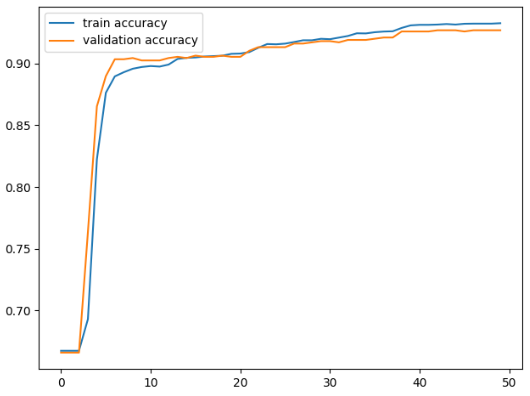
\includegraphics[scale=0.5]{mlp}
\caption{História učenia MLP modelu}
\end{figure}

Naše celkové výsledky teda vyzerajú nasledovne:
\begin{center}
\begin{tabular}{ |c|c|c|c|c| } 
 \hline
  prístup & baseline & SVC & RFC & MLP \\ 
  \hline
  úspešnosťou & 65\% & 95\% & 93.8\% & 93\% \\ 
  
 \hline
\end{tabular}
\end{center}


\section*{Záver}
V našom projekte sme sa venovali problematike klasifikácie phishingových mailov. Preskúmali sme niekoľko prístupov strojového učenia na nami vyextrahovaných vlastnostiach jednotlivých mailov z verejne dostupných datasetov. Dospeli sme k záveru, že konzistentne najlepšie výsledky dosahoval prístup SVC. Tieto výsledky sa samozrejme dajú zlepšiť pridaní ďalších features, ktoré by zlepšili presnosť klasifikátorov. V tomto projekte je priestor na ďalší rozvoj napríklad zostrojenie addonu do prehliadača, ktorý by vedel používateľa varovať pred niektorými podozrivými mailami.


\end{document}